\part{Capitulo 1}

\section{El Agua}

El agua es el recurso mas importante y con mayor abundancia del planeta.
Aun asi, su consumo se multiplico por 6 durante el siglo XX.

Algunos datos:

\begin{itemize}
    \item 97.5\% del agua es salada
    \item 2.5\% es dulce
    \item 70\% de esta agua dulce esta en forma de hielo
    \item 30\% esta en acuiferos
    \item 0.3\% esta en rios y lagos
    \item 70\% de la superficie del planeta es agua
    \item 69\% del agua es utilizada en el sector agropecuario
    \item 19\% en la industria
    \item 12\% en el sector municipal
\end{itemize}

\subsection{Uso del Agua en Chile}

\begin{itemize}
    \item 73\% del agua es utilizada en la agricultura
    \item 12\% en la industria
    \item 9\% en la mineria
    \item 6\% en el sector sanitario
\end{itemize}

\section{Hidrologia}

La Hidrología es la ciencia que trata de las aguas de la
Tierra, su existencia, circulación y distribución, sus
propiedades físicas, químicas y sus reacciones con el medio
ambiente, incluyendo su relación con los organismos vivos

\subsection{Objetivos}

\begin{itemize}
    \item Determinacion de la disponibilidad de recursos hidricos
    \item Efectuar estudios de crecidas
\end{itemize}

\section{Ciclo Hidrologico}

\begin{figure}[H]
    \centering
    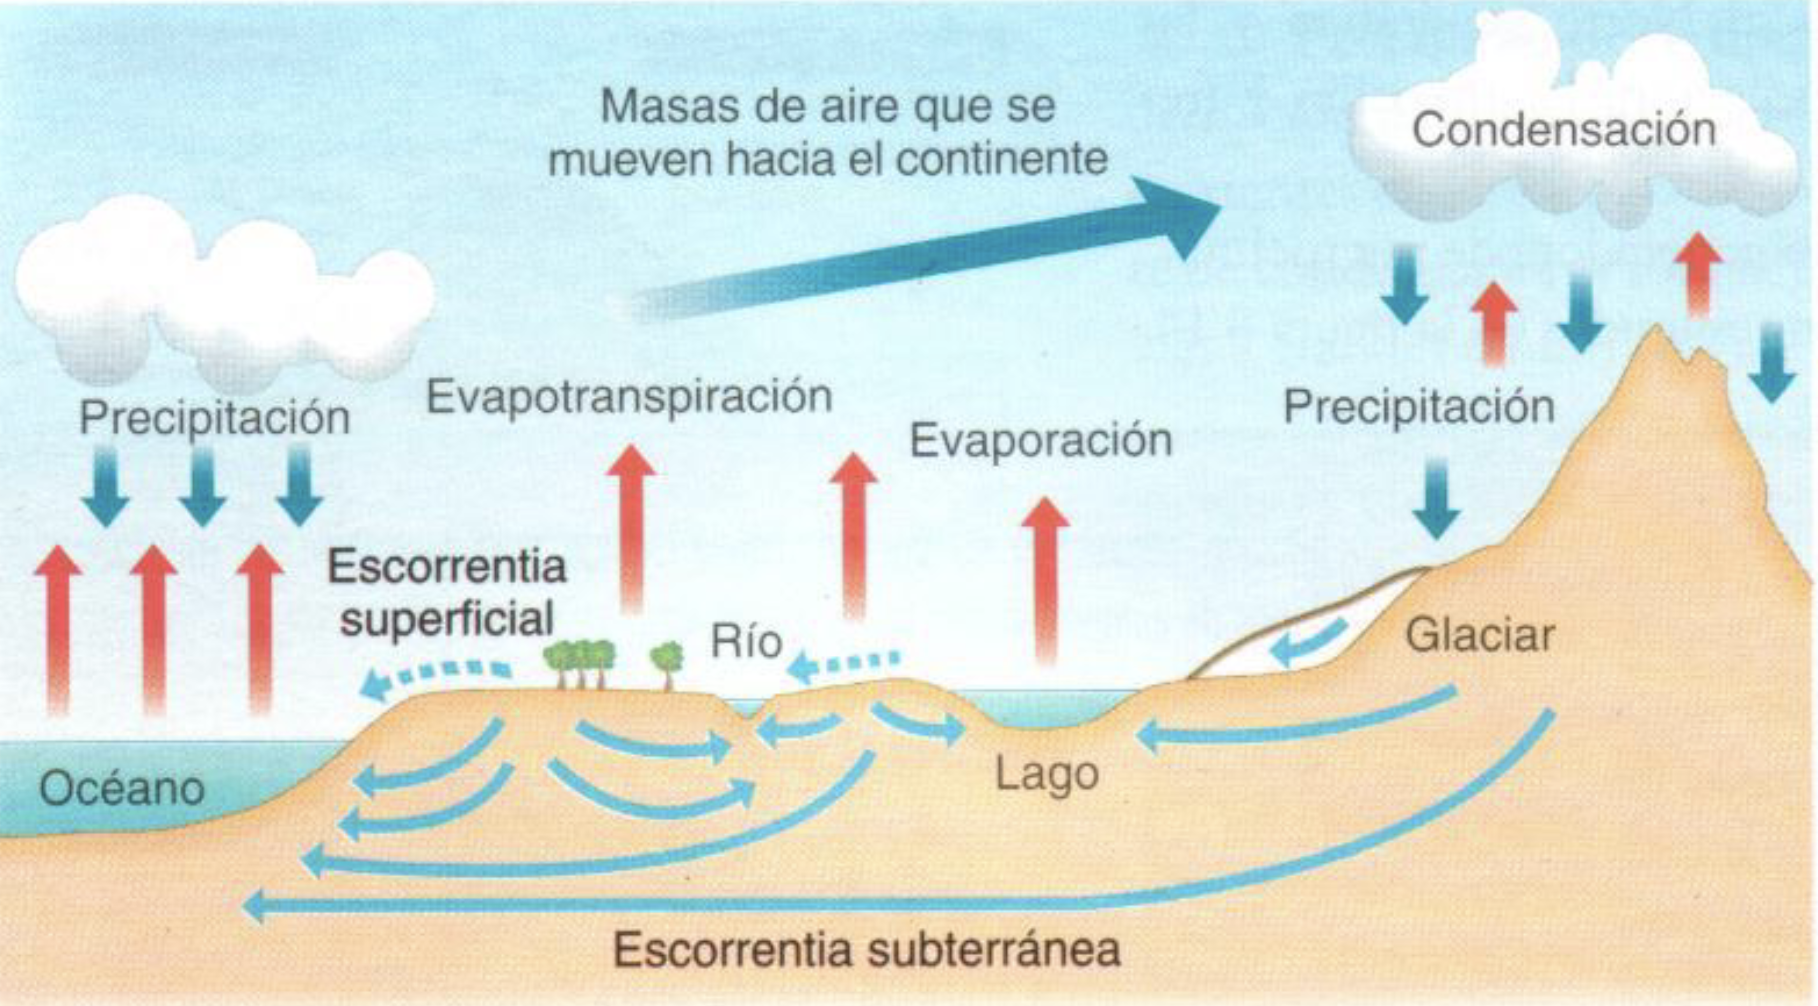
\includegraphics[width=0.85\textwidth]{imagenes/ciclo_hidrologico.png}
    \label{fig:ciclo_hidrologico}
\end{figure}

Se determina la precipitacion como \textbf{Pp}, evaporacion como \textbf{Ev} y la escorrentia como \textbf{Pp-Ev}.